\documentclass[11pt]{article}
\usepackage[margin=0.85in]{geometry}
\usepackage{amsmath,amssymb}
\usepackage{booktabs}
\usepackage{enumitem}
\usepackage{tikz}
\usetikzlibrary{positioning}
\usepackage[hidelinks]{hyperref}
\usepackage{titlesec}
\titlespacing*{\section}{0pt}{1.4ex plus 0.5ex}{0.7ex}
\setlist{nosep,leftmargin=1.4em}
\setlength{\parskip}{3pt}
\setlength{\parindent}{0pt}

\title{\vspace{-1.5em}Certified Conditional Cooperation Between Programs:\\ What We Tried, What We Learned, and When to Return}
\author{Findings memo for Cam and collaborators \quad (\texttt{\~{}/dev/diag}, November 2026)}
\date{\vspace{-2.5em}}

\begin{document}
\maketitle

\begin{center}
\fbox{\parbox{0.94\linewidth}{\small
\textbf{Status: parked.} We built a machine-checked scheme in which programs cooperate in the Prisoner's Dilemma by exchanging proof certificates, and it works. Its guarantees, however, rest on an assumption that program-equilibrium results usually leave implicit: a \emph{binding executor} that runs the code each player shows and delivers both moves. With such an executor, a plain escrow contract already gives the same guarantees. Without one, the fair-exchange impossibility applies, and the best any scheme can do is an $\varepsilon$ of exploitability. Our approach would matter only where execution is binding but there is no shared contract and each agent keeps its own code. We could not name such a setting. \emph{Return if someone can} (Section~5).}}
\end{center}

\section*{1\quad The goal}

Open-source game theory studies agents that read each other's source code before acting. In the one-shot Prisoner's Dilemma (payoffs $T > R > P > S$: temptation, reward, punishment, sucker), reading source makes \emph{conditional} cooperation possible. The best-known example is FairBot, which cooperates if it can prove that its opponent cooperates with it. By Löb's theorem, two FairBots cooperate even when written differently. The catch is that FairBot must \emph{search} for that proof. Exhaustive search over proofs of $B$ symbols costs about $|\Sigma|^B$ steps, so even $2^{128}$ steps reach only $B \approx 20$--$28$, while the proofs in Critch's bounded version of Löb's theorem need $B \gtrsim 10^4$.

Our idea was to replace search with checking, as in proof-carrying code. Players agree in advance on a \emph{standard} $K$, and each submits its program together with a \emph{certificate}: a proof that the program satisfies $K$. An LLM would write both, and at play time each side would run one certificate check and no search.

\section*{2\quad What we built}

The difficulty is self-reference. $K$ must say ``I cooperate with you exactly when your certificate proves that \emph{you} satisfy $K$.'' Naive versions either regress (a proof about a proof about\ldots) or fall into the \emph{Löb trap}: if the logic may reason about its own checker, every program becomes a member, including DefectBot, which always defects. We avoid both by defining $K$ with the diagonal lemma rather than Löb's theorem, and by giving our small object logic $S$ no reflection rule about its own checker.

The following are machine-checked in Lean~4, with no \texttt{sorry} and only Lean's three standard axioms.\footnote{Programs are written in a small DSL run by one fuel-bounded interpreter \texttt{run}, used both for the semantics and for play. The checker is \texttt{check}, with soundness \texttt{check\_sound}. The main results are \texttt{theoremA}, \texttt{theoremB}, \texttt{theoremA'}, \texttt{theoremB'} and \texttt{exclusivity\_unconditional}. CertBot's certification and its tournament outcomes are kernel-checked with \texttt{unseal} and \texttt{decide +kernel}, with no \texttt{native\_decide} or \texttt{\#eval} (\texttt{Diag/KernelChecked.lean}). The \texttt{\#print axioms} output is in \texttt{PROGRESS.md}, and the LLM pilot is in \texttt{m6/REPORT.md}.} The checker is sound. Within fixed size caps, two certified members cooperate (Theorem~A), and a certified member is never exploited (Theorem~B). A one-way variant $K'$ requires only the ``if'' direction, so even CooperateBot qualifies, and no program satisfies both $K$ and $K'$. Standards also do not interoperate: the $K$ and $K'$ versions of our reference member, CertBot, each check the other's certificate against their own standard, and so defect against each other, although both are ``cooperative.''

The following are measured, not proved. Certificates range from about 1.7k to 50k nodes, and a game takes about 5\,ms. In a pilot, an LLM wrote 8 of 8 certified members (6 on the first attempt), and the checker accepted none of 6 adversarial candidates. The generator was the same model that built the system, so the pilot is not independent evidence.

Building it taught us two technical lessons. First, $K$ can only quantify over opponents within fixed size caps, so ``certified'' must mean \emph{the checker accepts and the entry is within the caps}. Our first LLM runner checked only the former and accepted an over-cap certificate, which the tournament exposed. Second, $S$ at first could not use a negated test (``if the check is false, defect''), because nothing said \texttt{check} returns a boolean; a small rule, proved sound, fixed it.

The construction works. What it lacked was a reason anyone would need it, and the rest of the project was a search for one.

\section*{3\quad Why we parked it}

The arguments in this section are on paper, not formalized.

\textbf{Necessity does not single out certificates.} We first tried to show that the approach is forced: if P $\neq$ NP, no fast agent is both \emph{fair} (cooperates whenever a short proof of the opponent's cooperation exists) and \emph{unexploitable}. Our Lean version reduced from SAT, but it took the two hard steps as hypotheses. One of them is false under our fixed fuel cap, and proving the other inside $S$ would have needed induction and many more sessions. That effort turned out to be beside the point. A short diagonal argument with Contrarian (``play the opposite of what you play against me'') shows, with no complexity assumption, that no agent whose runs have short proofs is both fair and unexploitable. The argument is folklore-level (Anderlini 1990; Barasz et al., \S5), and it constrains \emph{every} feasible approach, so it cannot argue for ours.

\textbf{Zero exploitability is not a requirement.} If necessity cannot justify our criteria, the criteria must justify themselves, and unexploitability does not. Oesterheld's $\varepsilon$-grounded FairBot is already an equilibrium: defecting against it earns about $\varepsilon T + (1-\varepsilon)P$, which is less than $R$ for small $\varepsilon$. What survives is what Theorems A and B say together, a \emph{verifiable conditional commitment}: ``I cooperate if and only if you make the same commitment.''

\textbf{Even that commitment needs an executor.} Theorems A and B, like every program-equilibrium result we know of, assume that the code each player shows is the code that runs and that both moves are delivered. Making that assumption explicit splits the problem in two (Figure~\ref{fig:executor}). \emph{With} a binding executor, such as a smart contract or a referee, a plain escrow contract (``both commit, then both cooperate'') already gives A and B; it is the mediator of Monderer and Tennenholtz. \emph{Without} one, a certified agent can block its own incoming channel. It never receives the other's certificate, so it defects, exactly as $K$ prescribes, while the other receives its certificate, cooperates, and is exploited. We call this the \emph{self-starvation attack}. Signed receipts only push the problem one level up. It is the fair-exchange impossibility (Even and Yacobi; Pagnia and Gärtner) in strategic form, and its known escapes, collateral and gradual release, cost an $\varepsilon$ of exploitability, the same price $\varepsilon$-grounding pays.

\begin{figure}[h]
\centering
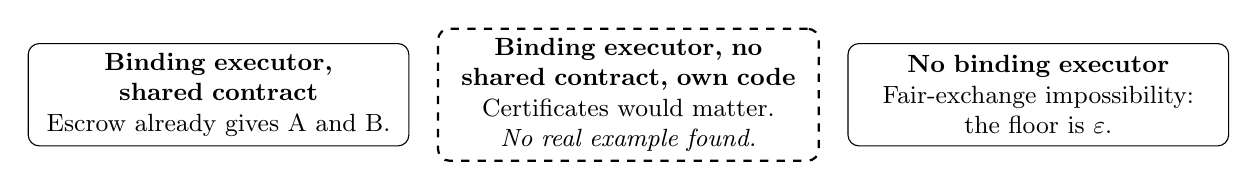
\begin{tikzpicture}[box/.style={draw,rounded corners,align=center,font=\small,text width=4.6cm,minimum height=1.3cm}]
\node[box] (a) {\textbf{Binding executor, shared contract}\\ Escrow already gives A and B.};
\node[box,right=0.35cm of a,dashed,thick] (b) {\textbf{Binding executor, no shared contract, own code}\\ Certificates would matter.\\ \emph{No real example found.}};
\node[box,right=0.35cm of b] (c) {\textbf{No binding executor}\\ Fair-exchange impossibility:\\ the floor is $\varepsilon$.};
\end{tikzpicture}
\caption{Where certificate-based cooperation could matter. Only the dashed regime distinguishes our approach, and we could not populate it.}
\label{fig:executor}
\end{figure}

So certificates have no regime of their own unless the middle box is occupied. That box is where our one distinctive feature, \emph{semantic membership}, would pay off: any program \emph{proved} to honor $K$ is a member, rather than one exact program (CliqueBot cooperates only with copies of itself) or one escrow address. The bare program-equilibrium model sits in the box by definition, but it is a model, not a deployment. The most plausible real candidate is on-chip governance commitments of the kind the flexHEG report proposes (Petrie et al.\ 2025): a chip commits to a policy ``if the other party makes the same commitment,'' which the authors call hard to build on-device. We have not examined it.

\section*{4\quad Paths to a paper}

Which paper exists, if any, depends on whether that box is occupied.

\textbf{If it stays empty: the hidden-assumption note.} Section~3's finding is itself the strongest result. Unexploitable conditional cooperation between programs \emph{is} fair exchange: with an executor, escrow suffices; without one, $\varepsilon$ is the floor; and Critch, Oesterheld and certificates become points on one map. The cooperative-AI literature lists checkable conditional commitments as open (for example, DiGiovanni, Clifton and Macé 2025 assume players can syntactically verify that a program follows an agreed template, and leave relaxing that to future work), so that audience may not know the reduction. But the charge that sinks the main line applies here too: cryptographers may consider it folklore. Our searches found no written version, but they were snippet-level and confabulated at least one source, so that absence is weak evidence.

\textbf{In either case: a theory note} for open-source game theory. Shipped proofs plus the diagonal lemma give cooperation with no proof search and no Löb, all machine-checked. It is modest, and the artifact exists. The nearest verified work is Duclaux et al.\ 2026 (Lean proofs of pairwise outcomes, written offline) and Ondras 2026 (a Lean handshake relying on a trusted attestation step). Peters and Szentes 2012 have diagonal contracts over program codes that match codes exactly rather than checking proofs (from our literature synthesis; not re-read).

\textbf{If the box is occupied: a full paper on the construction.} That paper would also need an LLM run with an independent model, and an answer to how different standards interoperate, since the $K$ and $K'$ versions of CertBot currently defect against each other.

\section*{5\quad When to pick this up}

\begin{center}
\small
\begin{tabular}{@{}p{0.38\linewidth}p{0.57\linewidth}@{}}
\toprule
\textbf{Resume if\ldots} & \textbf{Cheapest test} \\
\midrule
A real setting has binding execution but no shared contract, and agents keep their own code & Spend 30 minutes trying to name one, starting with flexHEG. Then ask whether one shared contract that runs an agreed program for both sides would serve instead. If it would, the case fails. \\
Nobody has written ``program equilibrium = fair exchange'' & One hour of searching, with opened sources only (Harrenstein 2007; Katz 1991; rational fair exchange), plus one email to Oesterheld or DiGiovanni. \\
Someone needs \emph{semantic} membership (any program proved to honor the standard), not template matching & Ask DiGiovanni, Clifton and Macé what relaxing their template assumption was meant to enable. \\
\midrule
\multicolumn{2}{@{}p{0.95\linewidth}@{}}{\textbf{Stop if} the reduction is already known \emph{and} no middle-regime setting turns up. Then archive the Lean repository and post, at most, a short note.}\\
\bottomrule
\end{tabular}
\end{center}

If we return, settle the criteria, and whether an executor is assumed, \emph{before} proving theorems. We did it the other way round, and most of our effort (the necessity theorem, about 135 literature searches) went to questions that do not bear on the open one. Treat any literature claim without an opened source as unverified. The Lean development, the literature corpus (\texttt{research/related\_work/}) and the record of every hypothesis we tried (\texttt{research/OUTLINE\_2026-11-18.md}) remain reusable.

\end{document}
